% -*- latex -*-
%%%%%%%%%%%%%%%%%%%%%%%%%%%%%%%%%%%%%%%%%%%%%%%%%%%%%%%%%%%%%%%%
%%%%%%%%%%%%%%%%%%%%%%%%%%%%%%%%%%%%%%%%%%%%%%%%%%%%%%%%%%%%%%%%
%%%%
%%%% This text file is part of the source of 
%%%% `Parallel Programming in MPI and OpenMP'
%%%% by Victor Eijkhout, copyright 2012-6
%%%%
%%%% mpi-morecollective.tex : obscure stuff
%%%%
%%%%%%%%%%%%%%%%%%%%%%%%%%%%%%%%%%%%%%%%%%%%%%%%%%%%%%%%%%%%%%%%
%%%%%%%%%%%%%%%%%%%%%%%%%%%%%%%%%%%%%%%%%%%%%%%%%%%%%%%%%%%%%%%%

\Level 0 {MPI Operators}

The following is the list of predefined \indexmpidef{MPI_OP} values.

\begingroup \tt\catcode`\_=12\relax
\begin{tabular}{ll}
  MPI_MAX&maximum\\
  MPI_MIN&minimum\\
  MPI_SUM&sum\\
  MPI_PROD&product\\
  MPI_LAND&logical and\\
  MPI_BAND&bitwise and\\
  MPI_LOR&logical or\\
  MPI_BOR&bitwise or\\
  MPI_LXOR&logical xor\\
  MPI_BXOR&bitwise xor\\
  MPI_MAXLOC&max value and location\\
  MPI_MINLOC&min value and location\\
\end{tabular}
\endgroup
All except the last two operate on MPI datatypes;
the last two operate on a value/index pair.

\Level 1 {User-defined operators}

In addition to the above predefined operators, the user can define new
operators to use in a reduction or scan operation.

\mpiRoutineRef{MPI_Op_create}

The function needs to have the following prototype:

\begin{verbatim}
typedef void MPI_User_function
    ( void *invec, void *inoutvec, int *len, 
      MPI_Datatype *datatype); 

FUNCTION USER_FUNCTION( INVEC(*), INOUTVEC(*), LEN, TYPE) 
<type> INVEC(LEN), INOUTVEC(LEN) 
INTEGER LEN, TYPE 
\end{verbatim}

The function has an array length argument~\n{len}, to allow for
pointwise reduction on a a whole array at once. The \n{inoutvec} array
contains partially reduced results, and is typically overwritten by
the function.

\Level 0 {Non-blocking collectives}
\label{sec:mpi3collect}

Above you have seen how the `Isend' and `Irecv' routines can overlap communication
with computation. This is not possible with the collectives you have seen so far:
they act like blocking sends or receives.
However, there are also \indextermsub{non-blocking}{collectives}.
These have roughly the same calling sequence as their blocking counterparts,
except that they output an \indexmpishow{MPI_Request}. You
can then use an \indexmpishow{MPI_Wait} call to make sure the collective
has completed.

Such operations can be used to increase efficiency.
For instance, computing
\[ y \leftarrow Ax + (x^tx)y \]
involves a matrix-vector product, which is dominated by computation
in the \indextermsub{sparse}{matrix} case, and an inner product which is 
typically dominated by the communication cost. You would code this as
\begin{verbatim}
MPI_Iallreduce( .... x ..., &request);
// compute the matrix vector product
MPI_Wait(request);
// do the addition
\end{verbatim}

This can also be used for 3D FFT operations~\cite{Hoefler:case-for-nbc}.
Occasionally, a non-blocking collective can be used for non-obvious purposes,
such as the \indexmpishow{MPI_Ibarrier} in~\cite{Hoefler:2010:SCP}.

The same calling sequence as the blocking counterpart, except for the addition
of an \indexmpishow{MPI_Request} parameter. For instance 
\indexmpishow{MPI_Ibcast}:
\begin{verbatim}
int MPI_Ibcast(
  void *buffer, int count, MPI_Datatype datatype,
  int root, MPI_Comm comm, 
  MPI_Request *request)
\end{verbatim}

\mpiRoutineRef{MPI_Iallreduce}

\mpiRoutineRef{MPI_Iallgather}

\Level 0 {Barrier and all-to-all}
\label{sec:barrier}
\label{sec:alltoall}

There are two collectives we have not mentioned yet. A~barrier is a
call that blocks all processes until they have all reached the barrier
call. This call's simplicity is contrasted with its usefulness, which
is very limited. It is almost never necessary to synchronize processes
through a barrier: for most purposes it does not matter if processors
are out of sync. Conversely, collectives (except the new non-blocking
ones) introduce a barrier of sorts themselves.

The all-to-all call is a generalization of a scatter and gather: every
process is scattering an array of data, and every process is gathering
an array of data. There is also a `v' variant of this routine.

\indexmpishow{MPI_Alltoall}
\begin{verbatim}
int MPI_Alltoall
  (void *sendbuf, int sendcount, MPI_Datatype sendtype, 
   void *recvbuf, int recvcount, MPI_Datatype recvtype, 
   MPI_Comm comm)
\end{verbatim}

\Level 0 {Reduce-scatter}
\label{reducescatter}

There are several MPI collectives that are functionally equivalent to
a combination of others. You have already seen \n{MPI_Allreduce} which
is equivalent to a reduction followed by a broadcast. Often such
combinations can be more efficient than using the individual calls;
see~\HPSCref{sec:collective}.

Here is another example: \indexmpishow{MPI_Reduce_scatter} is equivalent
to a reduction on an array of data (meaning a pointwise reduction on each
array location) followed by a scatter of this array to the individual 
processes.

One important example of this command is the
\indextermsub{sparse}{matrix-vector product};
see~\HPSCref{sec:spmvp-performance} for background information.
Each process contains one or more matrix rows, so by looking at indices
the process can decide what other processes it needs data from.
The problem is for a process to find out what other processes 
it needs to send data to. 

Using \indexmpishow{MPI_Reduce_scatter} the process goes as follows:
\begin{itemize}
\item Each process creates an array of ones and zeros, describing who
  it needs data from.
\item The reduce part of the reduce-scatter yields an array of
  requester counts; after the scatter each process knows how many
  processes request data from it.
\item Next, the sender processes need to find out what elements are
  requested from it. For this, each process sends out arrays of
  indices.
\item The big trick is that each process now knows how many of these
  requests will be coming in, so it can post precisely that many
  \n{MPI_Irecv} calls, with a source of \indexmpishow{MPI_ANY_SOURCE}.
\end{itemize}

The \indexmpishow{MPI_Reduce_scatter} command is equivalent to a reduction
on an array of data, followed by a scatter of that data to the individual processes.

To be precise, there is an array \n{recvcounts} where \n{recvcounts[i]} gives
the number of elements that ultimate wind up on process~\n{i}.
The result is equivalent to doing a reduction with a length equal to the sum
of the \n{recvcounts[i]} values, followed by a scatter where process~\n{i}
receives \n{recvcounts[i]} values. (Since the amount of data to be scattered
depends on the process, this is in fact equivalent to \indexmpishow{MPI_Scatterv}
rather than a regular scatter.)
%
\mpiRoutineRef{MPI_Reduce_scatter}
%
For instance, if all \n{recvcounts[i]} values are~1, the sendbuffer has one element
for each process, and the receive buffer has length~1.

\Level 1 {Examples}

An important application of this is establishing an irregular
communication pattern.  Assume that each process knows which
other processes it wants to communicate with; the problem is to
let the other processes know about this.
The solution is to use \n{MPI_Reduce_scatter} to find out how many processes
want to communicate with you, and then wait for precisely that many messages
with a source value of \indexmpishow{MPI_ANY_SOURCE}.
\verbatimsnippet{reducescatter}

Use of \n{MPI_Reduce_scatter} to implement the two-dimensional
matrix-vector product.
Set up separate row and column communicators with
\indexmpishow{MPI_Comm_split}, use \n{MPI_Reduce_scatter} to combine
local products.
%
\verbatimsnippet{mvp2d}

\Level 0 {Performance of collectives}

It is easy to visualize a broadcast as in figure~\ref{fig:bcast-simple}:
see figure~\ref{fig:bcast-simple}.
\begin{figure}[ht]
  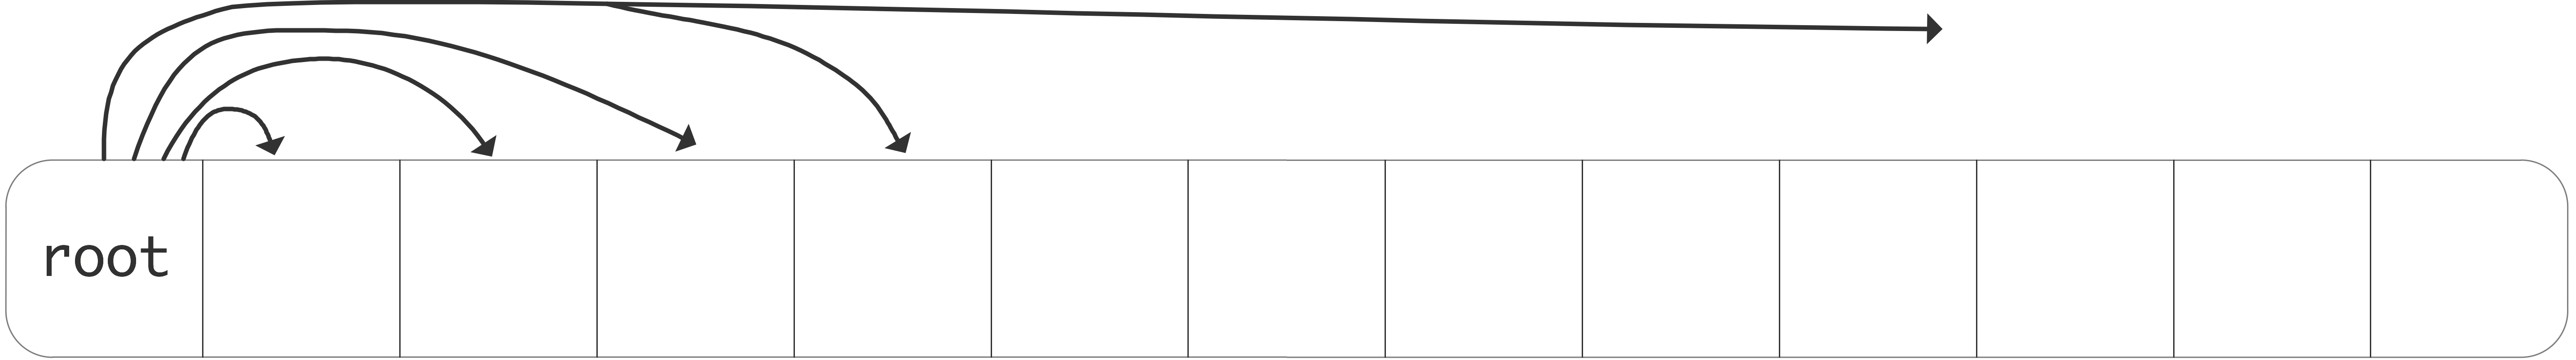
\includegraphics[scale=.08]{graphics/bcast-simple}
  \caption{A simple broadcast}
  \label{fig:bcast-simple}
\end{figure}
the root sends all of its data directly to every other process.
While this describes the semantics of the operation, in practice
the implementation works quite differently.

The time that a message takes can simply be modeled as
\[ \alpha +\beta n, \]
where $\alpha$~is the \indexterm{latency}, a~one time
delay from establishing the communication between two processes,
and $\beta$~is the time-per-byte, or the inverse of the \indexterm{bandwidth},
and $n$~the number of bytes sent.

Under the assumption that
a processor can only send one message at a time,
the broadcast in
figure~\ref{fig:bcast-simple} would take a time proportional to the
number of processors. One way to ameliorate that is to structure the
broadcast in a tree-like fashion.
\begin{figure}[ht]
  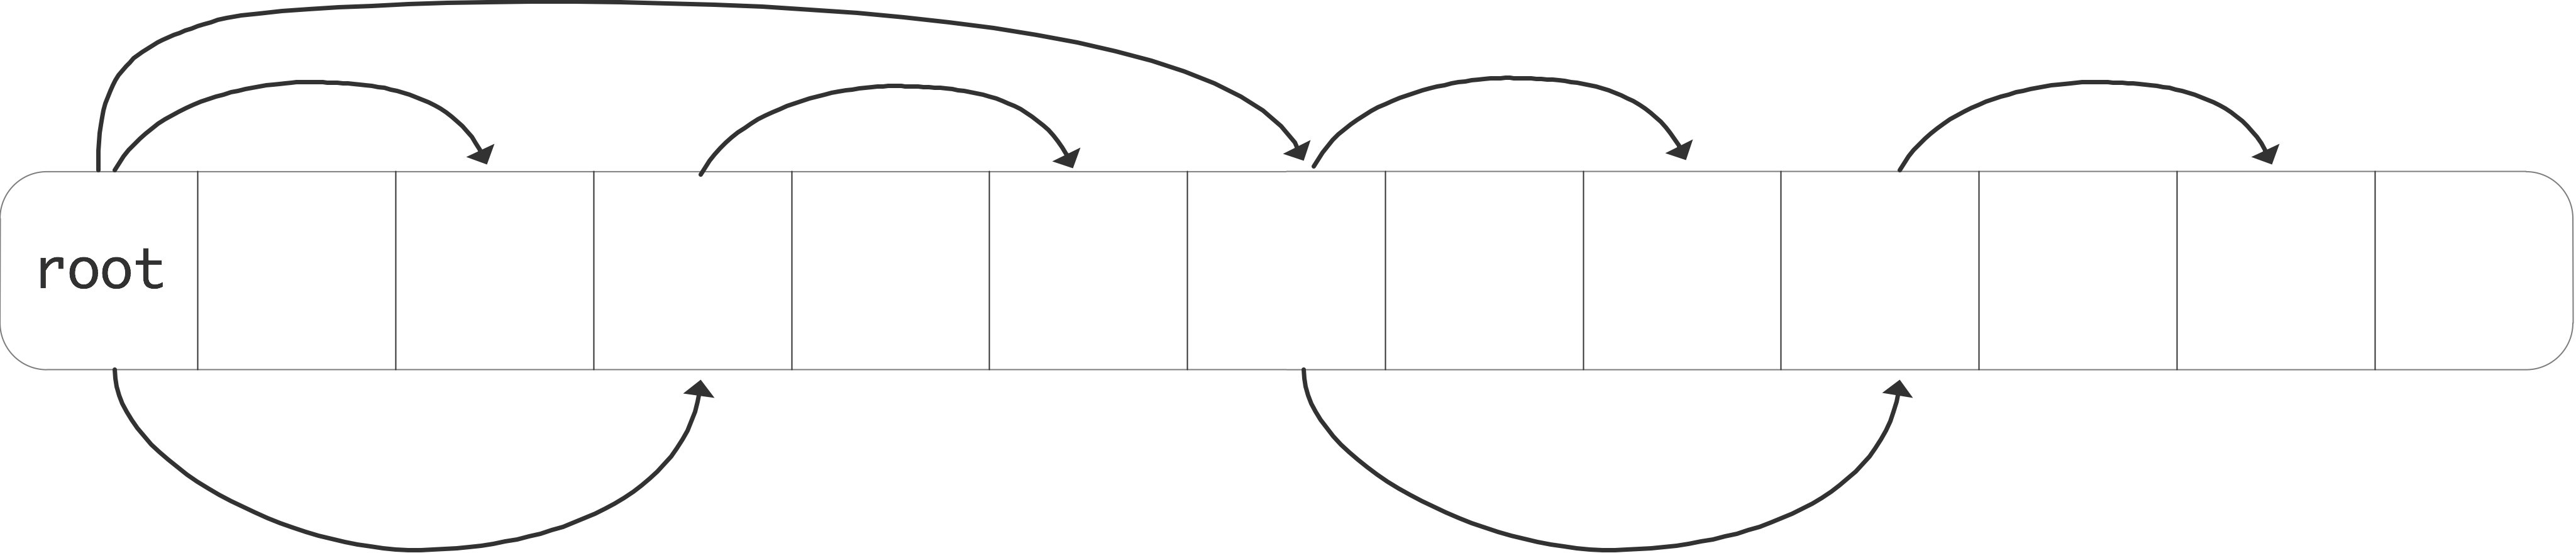
\includegraphics[scale=.1]{graphics/bcast-tree}
  \caption{A tree-based broadcast}
  \label{fig:bcast-tree}
\end{figure}
This is depicted in figure~\ref{fig:bcast-tree}. How does the
communication time now depend on the number of processors? The theory
of the complexity of collectives is described in more detail in
\HPSCref{sec:collective}; see also~\cite{Chan2007Collective}.

\Level 0 {Collectives and synchronization}

Collectives, other than a barrier, have a synchronizing effect between processors.
For instance, in
\begin{verbatim}
MPI_Bcast( ....data... root);
MPI_Send(....);
\end{verbatim}
the send operations on all processors will occur after the root executes
the broadcast. 
\begin{figure}[ht]
  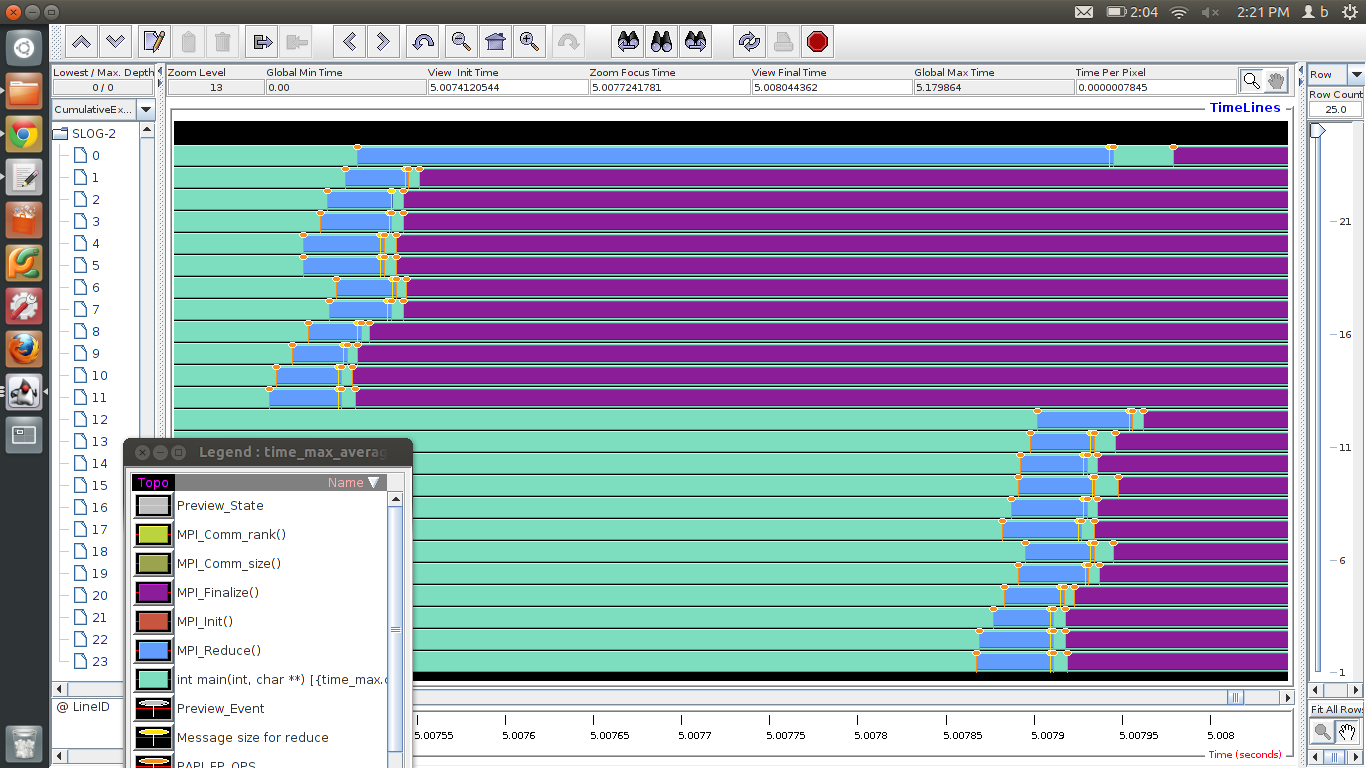
\includegraphics[scale=.35]{graphics/reduce-two-node}
  \caption{Trace of a reduction operation between two dual-socket 12-core nodes}
  \label{fig:trace-reduce}
\end{figure}
Conversely, in a reduce operation the root may have to wait for 
other processors. This is illustrated in figure~\ref{fig:trace-reduce}, which 
gives a TAU trace of
a reduction operation on two nodes, with two six-core sockets (processors) each.
We see that\footnote
{This uses mvapich version 1.6; in version 1.9 the implementation of an on-node reduction
has changed to simulate shared memory.}:
\begin{itemize}
\item In each socket, the reduction is a linear accumulation;
\item on each node, cores zero and six then combine their result;
\item after which the final accumulation is done through the network.
\end{itemize}
We also see that the two nodes are not perfectly in sync, which is normal for MPI
applications. As a result, core~0 on the first node will sit idle until it receives the partial
result from core~12, which is on the second node.

While collectives synchronize in a loose sense, it is not possible to
make any statements about events before and after the collectives
between processors:
\begin{verbatim}
...event 1...
MPI_Bcast(....);
...event 2....
\end{verbatim}
Consider a specific scenario:
\begin{verbatim}
switch(rank) { 
    case 0: 
        MPI_Bcast(buf1, count, type, 0, comm); 
        MPI_Send(buf2, count, type, 1, tag, comm); 
        break; 
    case 1: 
        MPI_Recv(buf2, count, type, MPI_ANY_SOURCE, tag, comm, status); 
        MPI_Bcast(buf1, count, type, 0, comm); 
        MPI_Recv(buf2, count, type, MPI_ANY_SOURCE, tag, comm, status); 
        break; 
    case 2: 
        MPI_Send(buf2, count, type, 1, tag, comm); 
        MPI_Bcast(buf1, count, type, 0, comm); 
        break; 
}
\end{verbatim}
Note the \n{MPI_ANY_SOURCE} parameter in the receive calls on processor~1.
One obvious execution of this would be:
\begin{enumerate}
\item The send from~2 is caught by processor~1;
\item Everyone executes the broadcast;
\item The send from~0 is caught by processor~1.
\end{enumerate}
However, it is equally possible to have this execution:
\begin{enumerate}
\item Processor~0 starts its broadcast, then executes the send;
\item Processor~1's receive catches the data from~0, then it executes
  its part of the broadcast;
\item Processor~1 catches the data sent by~2, and finally processor~2
  does its part of the broadcast.
\end{enumerate}

